
\documentclass{bmstu}[a4paper]
\renewcommand\labelitemi{--}
\usepackage[T1]{fontenc}

\usepackage{threeparttable}
\usepackage{diagbox}
\usepackage{rotating}
\usepackage{float} % Add this package for the H parameter
% ---------------------- Документ ----------------------
\bibliography{biblio}
\begin{document}

	\makecourseworktitle	
	{Информатика и системы управления} % Название факультета
	{Программное обеспечение ЭВМ и информационные технологии} % Название кафедры
	{Проектирование БД системы обогащения обучающей выборки для автоматизированной проверки отчета на соответствие нормативным требованиям} % Тема работы
	{Разин~А.В./ИУ7-64Б} % Номер группы/ФИО студента (если авторов несколько, их необходимо разделить запятой)
	{Строганов~Ю.~В.} % ФИО научного руководителя
	{} % ФИО консультанта (необязательный аргумент; если консультантов несколько, их необходимо разделить запятой)
	
	\setcounter{page}{3}
	\maketableofcontents

	\chapter*{ВВЕДЕНИЕ}
\addcontentsline{toc}{chapter}{ВВЕДЕНИЕ}

Во время обучения студентам регулярно приходится писать отчеты к различным видам работ (курсовые, лабораторные, научно-исследовательские работы и т. д.), при этом оформление работ должно соответствовать ГОСТ, что необходимо своевременно проверить и при необходимости отправить отчет на доработку, однако, количество студентов намного превышает количество нормоконтроллеров. Для ускорения процесса проверки возможно использование автоматических систем.

Целью курсовой работы является разработка базы данных обогащения обучающей выборки для автоматизированной проверки отчета на соответствие нормативным требованиям.

Для достижения цели научно-исследовательской работы требуется решить следующие задачи:
\begin{itemize}
	\item проанализировать существующие решения;
	\item формализовать задачу и определить необходимый функционал;
	\item проанализировать способы хранения данных и системы управления базами данных, выбрать подходящую систему для поставленной цели;
	\item спроектировать базу данных, описать ее сущности и связи;
	\item спроектировать и разработать базу данных;
	\item исследовать зависимость времени выполнения запроса от числа получаемых запросов;
\end{itemize}
	
\chapter{Аналитическая часть}
В данной части работы будет описаны ошибки в отчетах, которые необходимо обнаружить, а также описаны участники процесса приема лабораторных работ, также будут описаны существующие средства автоматизации.

\section{Основные ошибки в отчетах}
Основные ошибки в отчетах описаны в приложении~\ref{app:Mist}.

\section{Прием лабораторных работ}
В не автоматизированной системе проверки отчетов на соответствие ГОСТ и дополнительным требованиям присутствуют две роли: студент, выполняющий некоторую работы, которая подразумевает написание отчета и нормоконтроллер, принимающий экспертное решение о соответствии предоставленного ему отчета необходимым требованиям.
\subsection{Участники процесса приема работ}
С помощью использования автоматической проверки отчета возможно
сократить временные ресурсы, выделяемые нормоконтроллером на проверку
отчетов студентов, однако, полностью отказаться от финального контроля
результатов человеком невозможно, таким образом существует две роли при
проверки отчета на соответствие ГОСТ, а именно: студент и нормоконтроллер.

\subsection{Процесс приема работ}

Студент отправляет отчет на проверку, а затем получает результат со
списком ошибок (если имеются). Нормоконтроллер же анализирует отчет,
составленный автоматической системой проверки, и при необходимости может
внести необходимые правки. Диаграммы процесса проверки отчетов приведены на картинках~\ref{img:ka}--\ref{img:stepsDiagram}, также приведена диаграмма BPMN~2.0, на которой представлено взаимодействие системы проверки отчетов, нормоконтроллера и студента~(рисунок \ref{img:user_inter}).

Использование автоматической проверки отчетов на соответствие ГОСТ и дополнительным требованиям сократит временные затраты на проверку отчетов.


\includeimage
{ka} % Имя файла без расширения (файл должен быть расположен в директории inc/img/)
{f} % Обтекание (без обтекания)
{H} % Положение рисунка (см. figure из пакета float)
{1\textwidth} % Ширина рисунка
{Диаграмма состояний проверки отчета} % Подпись рисунка

\includeimage
{stepsDiagram} % Имя файла без расширения (файл должен быть расположен в директории inc/img/)
{f} % Обтекание (без обтекания)
{H} % Положение рисунка (см. figure из пакета float)
{0.8\textwidth} % Ширина рисунка
{Диаграмма последовательности действий} % Подпись рисунка

\includeimage
{user_inter} % Имя файла без расширения (файл должен быть расположен в директории inc/img/)
{f} % Обтекание (без обтекания)
{H} % Положение рисунка (см. figure из пакета float)
{1\textwidth} % Ширина рисунка
{BPMN 2.0 диаграмма сдачи лабораторной работы} % Подпись рисунка


\section{Формализация требований к базе данных и приложению}
В ходе выполнения курсовой работы необходимо разработать базу данных для хранения информации о студентах их работ, достижениях и результатов проверки работ студентов, также стоит хранить разметку основных частей отчетов студентов.

Необходимо спроектировать и разработать приложение, которое позволит проверять отчеты студентов, сохранять их, а также сохранять новые разметки основных частей отчета.


\section{Анализ существующих средств автоматизации}
Ввиду распространенности решаемой проблемы уже были созданы приложения для автоматизации проверки документов на соответствие стандартам.

Наиболее популярными из них являются:
\begin{enumerate}
	\item ВКР-СМАРТ~\cite{VKR_VYZ};
	\item TestVkr~\cite{TestVkr};
	\item Applitools visual testing~\cite{PdfTest};
\end{enumerate}

Система ВКР-СМАРТ, предназначенная для проверки выпускных квалификационных работ (ВКР) студентов, представляет собой универсальную платформу, разработанную для системного хранения и проверки на заимствования ВКР и других работ обучающихся. Также система проверяет предложенные работы на выполнение всех требований ФГОС ВО и СПО, а также соответствие ГОСТам. После выполнения проверок, будет получен отчет о проценте заимствования и замечания по нарушенным стандартам~\cite{VKR_VYZ}.

Система ТЕСТ ВКР (Технический регламент проверки выпускных квалификационных работ) предназначена для проверки выпускных квалификационных работ студентов на объем заимствования и их размещения в электронно-библиотечной системе (ЭБС) университета. Система обеспечивает централизованное хранение и контроль за академическими работами студентов, а также их проверку на оригинальность и уникальность контента, также данную систему (без использования хранилища) возможно запускать локально, для проверки работы на нарушение ГОСТ~\cite{TestVkr}.

Платформа Applitools позволяет использовать <<визуальное тестирование>> предназначенное для сравнения получаемого изображения с реальным. Этот метод особенно эффективен при выявлении ошибок во внешнем виде страницы или экрана, которые могут остаться незамеченными при традиционном функциональном тестировании. С использованием Applitools Eyes разработчики могут легко интегрировать визуальные тесты, которые могут быть использованы для выявления отклонений от стандартов в PDF~\cite{PdfTest}.



\begin{table}[ht]
	\begin{center}
		\begin{threeparttable}
			\caption{\label{t:cmp} Сравнение существующих средств автоматизации}
			\begin{tabular}{|p{4cm}|p{4cm}|p{4cm}|c|}
				\hline
				\textbf{Критерий} & \textbf{ВКР СМАРТ} & \textbf{TestVkr} & \textbf{Applitools} \\ \hline
				Проверка текстов  & да & да & нет\\ \hline
				Проверка элементов отчета & нет & нет & да \\ \hline
				Наличие общего хранилища работ  & да & да & нет \\ \hline
				Возможность запуска локально & нет & *да & *да \\ \hline
			\end{tabular}
		\end{threeparttable}
	\end{center}
\end{table}


В таблице~\ref{t:cmp} под <<элементами отчета>> подразумеваются таблицы, рисунки, схема алгоритмов, формулы, использование символа *, означает, что в этом случае проверка плагиата не производится.

\section{Формализация информации, подлежащей хранению в проектируемой базе данных}
Разрабатываемая база данных, должна содержать информацию о следующих сущностях:
\begin{itemize}
	\item студент;
	\item нормоконтроллер;
	\item отчет студента;
	\item тип фрагмента отчета;
	\item фрагмент отчета;
	\item комментарий студента;
	\item достижение студента.
\end{itemize}

Сведения о каждой категории данных содержится в таблице~\ref{t:data_store}.

\begin{table}[ht]
	\begin{center}
		\begin{threeparttable}
			\caption{\label{t:data_store} Категории и сведения о данных}
			\begin{tabular}{|c|p{8cm}|}
				\hline
				\textbf{Категория} & \textbf{Сведения} \\ \hline
				Студент & ID источника данных, ID студента, никнейм, имя, фамилия, дата регистрации, число сданных лабораторных\\ \hline
				Отчет & ID отчета, номер попытки сдачи, файл отчета, время последнего обновления отчета, число проверок отчета, ID студента, значение того что отчет сдан \\ \hline
				Тип фрагмента отчета & ID фрагмента, описание типа фрагмента, ID контроллера, создавшего фрагмент отчета \\ \hline
				Выделенный фрагмент отчета & ID фрагмента отчета, изображение страницы отчета, данные фрагмента отчета (разметка), значение была ли ошибка проверена разметчиком, ID отчета, ID типа фрагмента отчета, ID проверяющего отчет\\ \hline
				Комментарий & ID ошибки, на которую создается комментарий, ID комментария, данные комментария, ID студента, создавшего комментарий \\ \hline
				Достижение & ID достижения, ID контроллера, создавшего достижение, данные достижения, описание достижения \\ \hline
			\end{tabular}
		\end{threeparttable}
	\end{center}
\end{table}

На основе описанной информации была получена диаграмма сущность---связь, представленная на рисунке~\ref{img:ER_RU}.
\includeimage
{ER_RU} % Имя файла без расширения (файл должен быть расположен в директории inc/img/)
{f} % Обтекание (без обтекания)
{H} % Положение рисунка (см. figure из пакета float)
{1\textwidth} % Ширина рисунка
{Диаграмма сущность---связь} % Подпись рисунка


\section{Анализ существующих баз данных}
База данных —-- это некоторый набор перманентных (постоянно хранимых) данных, используемых прикладными программными системами какого-либо предприятия~\cite{williams-db}.

Между физической базой данных (т.е. данными, которые реально хранятся на компьютере) и пользователями системы располагается уровень программного
обеспечения, который можно называть по-разному: диспетчер базы данных (database 
manager), сервер базы данных (database server) или, что более привычно, система управления базами данных, СУБД (DataBase Management System — DBMS).
Основная задача СУБД --- дать пользователю базы данных возможность работать с ней, не вникая во все подробности работы на уровне аппаратного обеспечения~\cite{williams-db}.

Модель данных — это абстрактное, самодостаточное, логическое определение объектов, операторов и прочих элементов, в совокупности составляющих абстрактную машину доступа к данным, с которой взаимодействует пользователь~\cite{williams-db}.
Рассмотрим классификацию баз данных по различным моделям данных:
\begin{enumerate}
	\item дореляционные;
	\item реляционные;
	\item постреляционные.
\end{enumerate}

\subsection{Дореляционные модели}
Дореляционные системы можно разделить на три большие категории:
\begin{enumerate}
	\item системы с инвертированными списками;
	\item иерархические;
	\item сетевые~\cite{williams-db}.
\end{enumerate}
Иерархическая база данных представляется множеством 
деревьев: в вершинах дерева помещаются записи, состоящие из поименованных 
полей и представляющие экземпляры некоторого объекта предметной области. 
Записи связаны строго иерархическими отношениями --- у записи-<<потомка>> не 
должно быть более одной записи-<<предка>>~\cite{wolf-db}.

Сетевая модель данных представляет собой логическую модель данных, которая расширяет иерархический подход. В иерархических структурах каждая запись-потомок имеет ровно одного предка, в то время как в сетевой структуре данных потомок может иметь несколько предков~\cite{wolf-db}.

Инвертированный список в общем случае — это двухуровневая индексная структура. На первом уровне находится файл или часть файла, в которой упорядоченно расположены значения вторичных ключей. Каждая запись с вторичным ключом имеет ссылку на номер первого блока в цепочке блоков, содержащих номера записей с данным значением вторичного ключа. На втором уровне находится цепочка блоков, содержащих номера записей, содержащих одно и то же значение вторичного ключа. При этом блоки второго уровня упорядочены по значениям вторичного ключа, на третьем уровне находится основной файл~\cite{inverted-lists}.

Механизм доступа к записям по вторичному ключу при подобной организации записей весьма прост. На первом шаге происходит поиск в области первого уровня заданное значение вторичного ключа, а затем по ссылке считываются блоки второго уровня, содержащие номера записей с заданным значением вторичного ключа, а далее уже прямым доступом загружается в рабочую область пользователя содержимое всех записей, содержащих заданное значение вторичного ключа~\cite{inverted-lists}.


\subsection{Реляционные модели}
Реляционная база данных — это такая база данных, которая воспринимается ее пользователями как множество переменных (т.е. переменных отношения), значениями которых являются отношения или, менее формально, таблицы~\cite{williams-db}.

Реляционная система, поддерживает реляционные базы данных и осуществляет операции над ними, включая RESTRICT (также известную как выборка или англ. SELECT), проекцию (англ. PROJECT) и соединение (англ. JOIN). Эти и подобные операции реляционной алгебры выполняются на уровне множеств~\cite{williams-db}.

\subsection{Постреляционные модели}
Современный (постреляционный) этап развития связан с использованием объектно-ориентированных технологий разработки программных систем и созданием СУБД нового поколения, унаследовавших все лучшее от дореляционных и реляционных систем. Постреляционные СУБД поддерживают 
объектные и объектно-реляционные модели данных и обеспечивают разработчикам возможность использовать объектно-ориентированные языки программирования, что дает таким системам технологические преимущества по сравнению с реляционными СУБД~\cite{wolf-db}.

\subsection{Хранение временных рядов}
Отдельно стоит отметить набирающие популярность СУБД временных рядов. Временные ряды (Time series) --- это данные, 
претерпевающие некоторые изменения с течением 
времени, и фиксируемые в конкретные промежутки 
времени. Данные СУБД оптимизированы под частую запись данных и скорость получения доступа к данным не настолько сильно зависит от числа хранимых данных, что характерно для реляционных баз данных, скорость работы которых уменьшается ввиду необходимости индексирования новых элементов. Однако во временных СУБД отсутствует механизм изменения записанных значений, так как считается что записанные метрики (данные) являются фактом в прошлом~\cite{time_db}.

\section*{Вывод}
В данном разделе были описаны основные ошибки студентов в отчетах по лабораторным работам, были выделены участники процесса приема лабораторных работ, формализован процесс приема лабораторных работ, а также рассмотрены существующие средства автоматизации проверки работ на соответствие стандартам.


	
\chapter{Конструкторская часть}
В данной части работы будет описана реализация базы данных, описана ER диаграмма БД и принципиальная схема БД, также будут описаны схемы триггеров и хранимые процедуры.


\section{Формализация взаимодействия с приложением}


Системе автоматической проверки необходимо проверить на правильность составные части отчета, что подразумевает детекцию рисунков, графиков, схем алгоритмов, списка используемых источников, а также формул.

На рисунках \ref{img:detection}--\ref{img:detection_inside} представлены результаты разработки системы детекции составных частей.

\includeimage
{detection} % Имя файла без расширения (файл должен быть расположен в директории inc/img/)
{f} % Обтекание (без обтекания)
{H} % Положение рисунка (см. figure из пакета float)
{1\textwidth} % Ширина рисунка
{IDEF0 обнаружение составных частей отчет 0 уровня} % Подпись рисунка

\includeimage
{detection_inside} % Имя файла без расширения (файл должен быть расположен в директории inc/img/)
{f} % Обтекание (без обтекания)
{H} % Положение рисунка (см. figure из пакета float)
{1\textwidth} % Ширина рисунка
{IDEF0 обнаружение составных частей отчета 1 уровня} % Подпись рисунка

После решения задачи детекции необходимо проверить составные части на соответствие ГОСТ 7.32, однако, финальный вердикт должен выноситься экспертом. На рисунках \ref{img:errors}--\ref{img:errors_inside} представлены результаты разработки данной системы.

\includeimage
{errors} % Имя файла без расширения (файл должен быть расположен в директории inc/img/)
{f} % Обтекание (без обтекания)
{H} % Положение рисунка (см. figure из пакета float)
{1\textwidth} % Ширина рисунка
{IDEF0 проверки составных частей отчета на соответствие ГОСТ 7.32 0 уровня} % Подпись рисунка

\includeimage
{errors_inside} % Имя файла без расширения (файл должен быть расположен в директории inc/img/)
{f} % Обтекание (без обтекания)
{H} % Положение рисунка (см. figure из пакета float)
{1\textwidth} % Ширина рисунка
{IDEF0 проверки составных частей отчета на соответствие ГОСТ 7.32 1 уровня} % Подпись рисунка
\newpage
\section{Формализация работы системы проверки отчета}
На рисунке~\ref{img:main_sys_bpmn}, представлена схема BPMN 2.0 работы системы в процессе проверки отчета, а также всех взаимодействующих с ней акторов.
\begin{sidewaysfigure}[H]
	\centering
	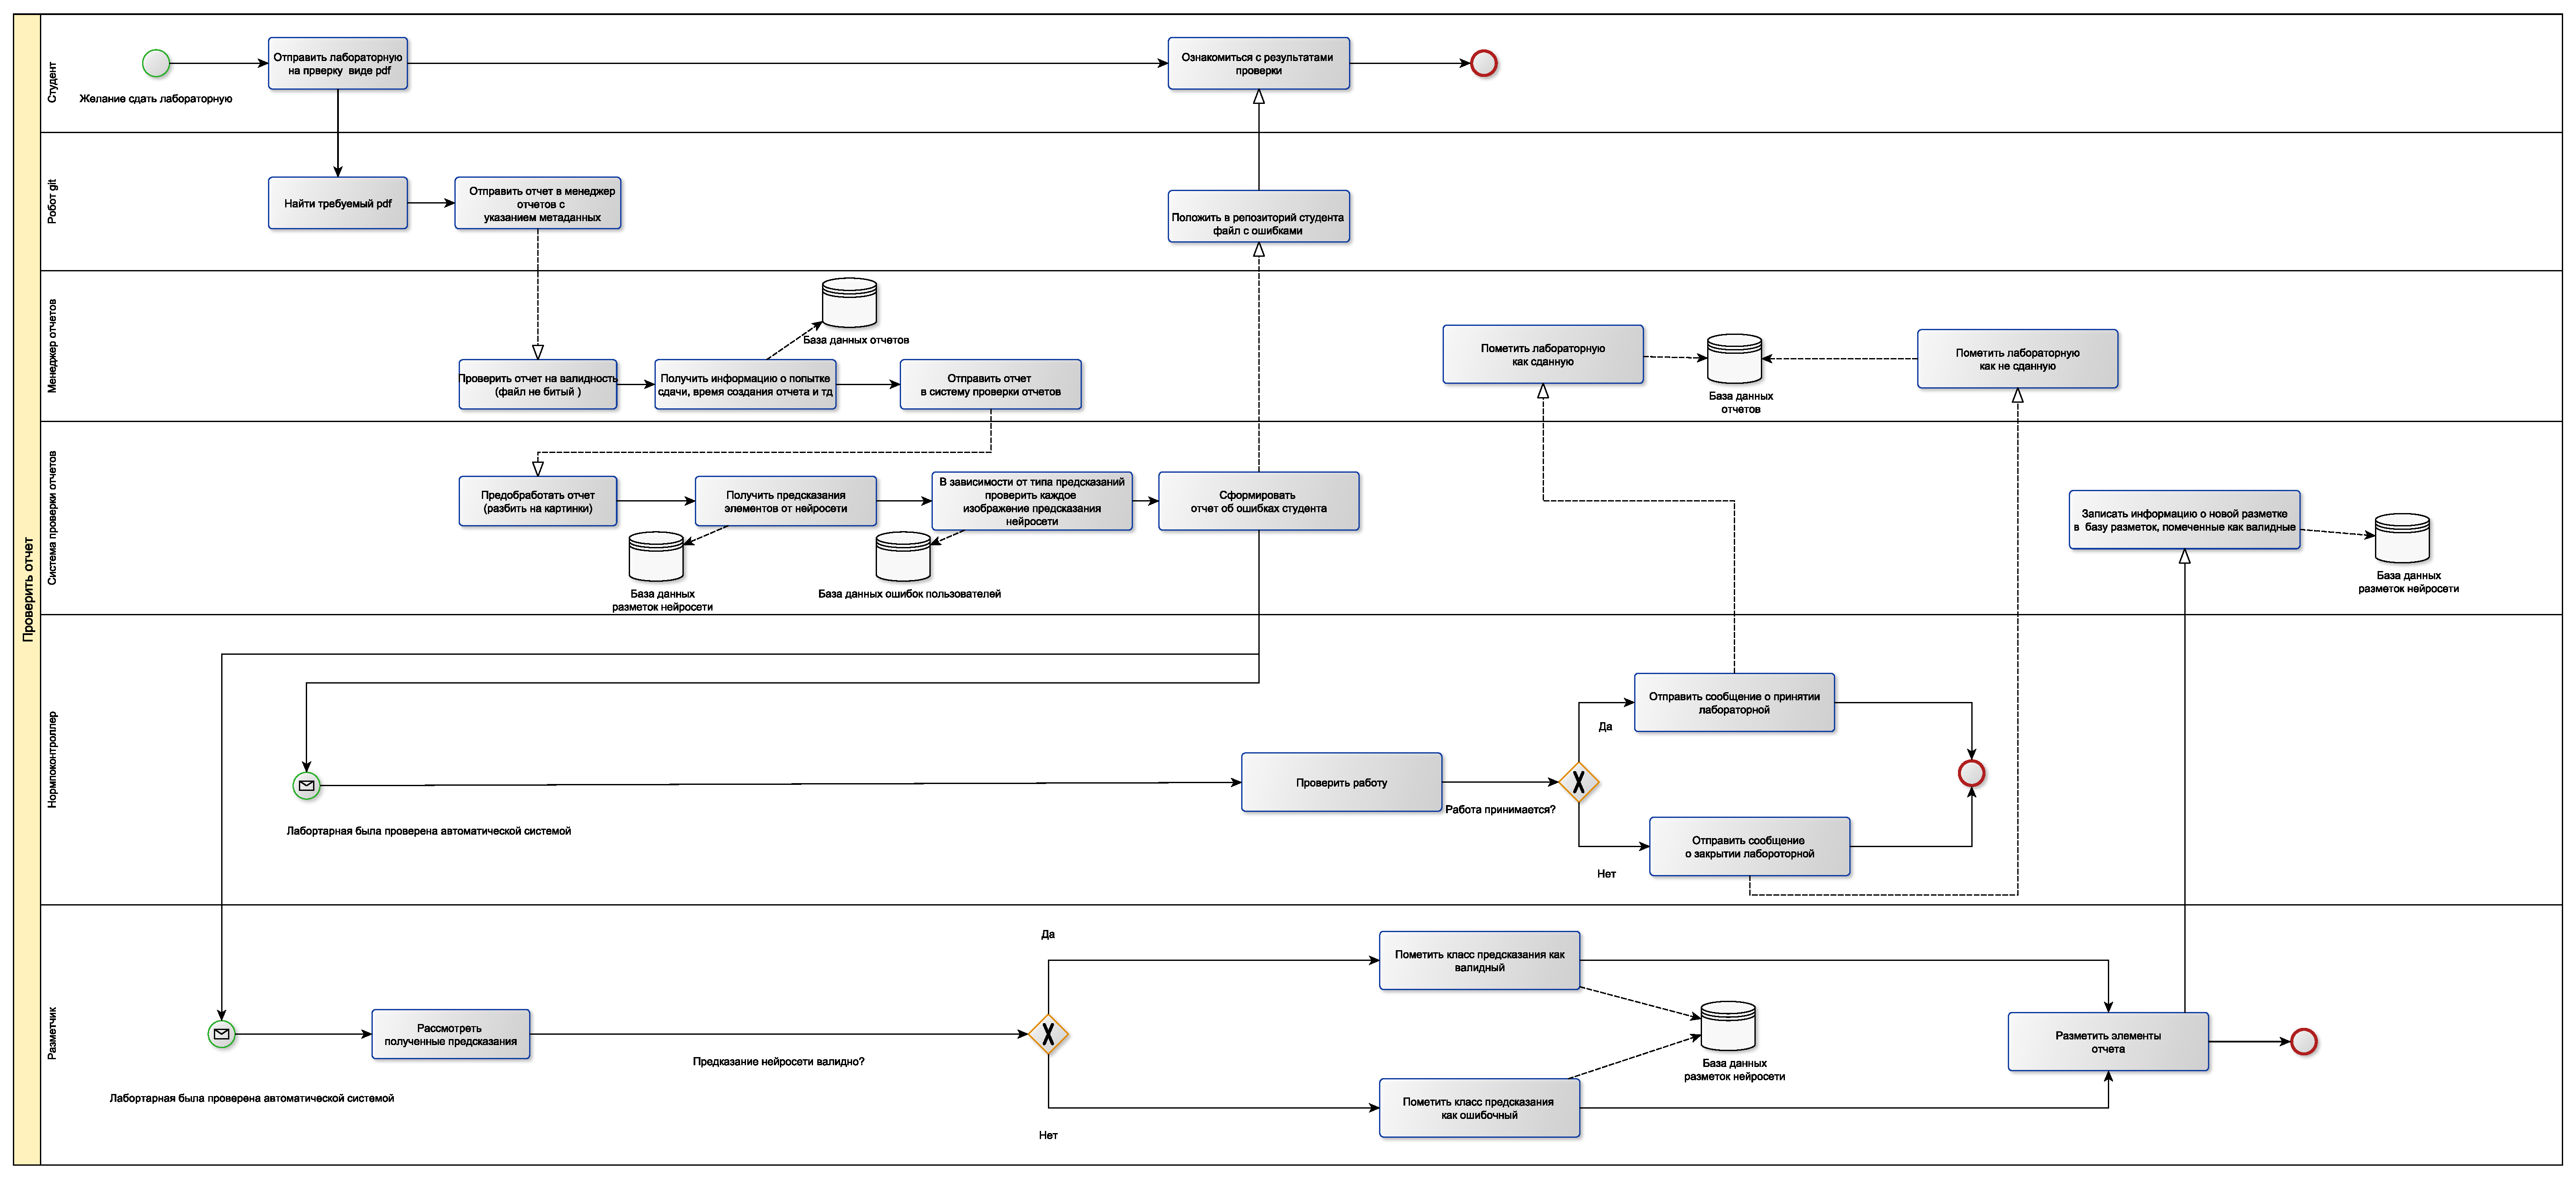
\includegraphics[width=\textwidth]{./inc/img/process_check_bpmn.pdf}
	\caption{Схема BPMN 2.0 работы системы}
	\label{img:main_sys_bpmn}
\end{sidewaysfigure}


\section{Формализация сущностей базы данных}

В соответствие с диаграммами~\ref{img:errors}--\ref{img:errors_inside} были выделены следующие таблицы:
\begin{enumerate}
	\item студент --- сущность студента (имеет уникальный идентификатор для связи со сданными отчетами и комментариями);
	\item нормоконтроллеер --- сущность нормоконтроллера (имеет уникальный идентификатор для связи с проверенными отчетами и созданными ошибками);
	\item выделенный фрагмент --- сущность ошибок в отчетах студентов (хранит страницу отчета с ошибкой, а также данные, указывающие на местоположение ошибки, а также тип фрагмента);
	\item тип фрагмента~---~сущность типов ошибок (необходима для введения новых типов ошибок, хранит описание ошибки);
	\item отчет --- сущность отчета студента (хранит все страницы попытки сдачи отчета, а также время сдачи и номер попытки сдачи);
	\item комментарий --- сущность комментария студента о ошибке (в случае ошибки преподавателя можно указать на это, кроме данных комментария хранит идентификатор студента, создавшего комментарий);
	\item достижение --- сущность награды для выдачи студентам, преуспевающим в выполнении лабораторных работ (хранит идентификатор студента, которому выдали награду, а также идентификатор отчета, за который было получено достижение).
\end{enumerate}

\section{Ограничения целостности базы данных}
В данной части работы будут описаны описаны поля сущностей баз данных и их ограничения, для обеспечения целостности данных системы. Ограничение <<первичный ключ>> подразумевает то что поле сущности является первичным ключом данного отношения в реляционной модели данных.
\begin{table}[h!tbp]
	\centering
	\caption{Ограничение целостности сущности отчета}
	\begin{tabularx}{\textwidth}{|X|X|X|}
		\hline
		Поле & Тип & Ограничение \\
		\hline
		id & целое число & первичный ключ \\
		\hline
		page\_count & целое число & не пустое значение\\
		\hline
		document\_name & строка & не пустое значение\\
		\hline
		checks\_count & целое число & не пустое значение\\
		\hline
		creator\_id & целое число & не пустое значение\\
		\hline
		creation\_time & дата и время & не пустое значение\\
		\hline
	\end{tabularx}

	\label{t:documents_cons}
\end{table}

\begin{table}[h!tbp]
	\centering
	\caption{Ограничение целостности сущности фрагмента}
	\begin{tabularx}{\textwidth}{|X|X|X|}
		\hline
		Поле & Тип & Ограничение \\
		\hline
	  	id & целое число & первичный ключ \\
	  	\hline
		description & строка & не пустое значение \\
		\hline
		creator\_id & целое число & не пустое значение\\
		\hline
		class\_name & строка & не пустое значение\\
		\hline
	\end{tabularx}
	
	\label{t:markup_type_cons}
\end{table}

\begin{table}[H]
	 \centering
	 \caption{Ограничение целостности сущности типа фрагмента}
	\begin{tabularx}{\textwidth}{|X|X|X|}
		\hline
		Поле & Тип & Ограничение \\
		\hline
		id & целое число & первичный ключ \\
		\hline
		page\_data & байты изображения & не пустое значение\\
		\hline
		error\_bb & массив из 4 вещественных чисел & не пустое значение\\
		\hline
		class\_label & целое число & не пустое значение\\
		\hline
		creator\_id & целое число & не пустое значение\\
		\hline
	\end{tabularx}
	\label{t:markups}
\end{table}




\begin{table}[h!tbp]
	\centering
	\caption{Ограничение целостности сущности пользователя}
	\begin{tabularx}{\textwidth}{|X|X|X|}
	\hline
	Поле & Тип & Ограничение \\
	\hline
	id & целое число & первичный ключ\\
	\hline
	login & строка & уникальный,не пустое значение\\
	\hline
	password & строка & не пустое значение\\
	\hline
	name & строка & не пустое значение\\
	\hline
	surname & строка & не пустое значение\\
	\hline
	role\_id & целое число & не пустое значение\\
	\hline
	role\_type & строка & не пустое значение\\
	\hline
	group & строка & не пустое значение\\
	\hline
	\end{tabularx}
	\label{t:users_cons}
\end{table}


\begin{table}[h!tbp]
	\centering
	\caption{Ограничение целостности сущности достижения}
	\begin{tabularx}{\textwidth}{|X|X|X|}
		\hline
		Поле & Тип & Ограничение \\
		\hline
		id & целое число & первичный ключ\\
		\hline
		picture & байты изображения &  не пустое значение\\
		\hline
		text & строка & не пустое значение\\
		\hline
		creator\_id & целое число & не пустое значение\\
		\hline
		granted\_to\_id & целое число & не пустое значение \\
		\hline
	\end{tabularx}
	\label{t:achievment_cons}
\end{table}

\begin{table}[h!tbp]
	\centering
	\caption{Ограничение целостности сущности комментария}
	\begin{tabularx}{\textwidth}{|X|X|X|}
		\hline
		Поле & Тип & Ограничение \\
		\hline
		id & целое число & первичный ключ\\
		\hline
		description & строка & не пустое значение\\
		\hline
		creator\_id & целое число & не пустое значение\\
		\hline
		report\_id & целое число & не пустое значение\\
		\hline
	\end{tabularx}
	\label{t:comment_cons}
\end{table}






\section{Ролевая модель}
Была определена следующая ролевая модель:
\begin{enumerate}
	\item Разметчик --- имеет права доступа SELECT к таблице документов и INSERT к таблице выделенных фрагментов.
	\item Добавляющий --- имеет права доступа INSERT к таблице студентов и нормоконтроллеров
	\item Пользователь --- имеет права доступа INSERT к таблице комментариев, имеет права доступа SELECT  и INSERT к таблице выделенных фрагментов.
	\item Нормоконтроллер --- является разметчиков, также имеет права доступа INSERT и SELECT к таблице тип\_ошибки и таблице достижений.
	\item Администратор имеет все права доступа ко всем таблицам.
	\item Также выделяется работник очереди задача которого --- работать с отчетами из очереди и помечать их как проверенные,имеет права доступа SELECT и UPDATE к очереди документов.
	\item При проверке документов из очереди система работает в роли работника очереди, в иных случаях система использует роль администратора.
\end{enumerate}

\section{Определение модели базы данных}
Необходимо определить модель базы данных, которая будет использована для хранения информации в системе. Реляционная модель баз данных позволяет хранить сущности в целостном виде и поддерживает сложные запросы, поэтому она является наилучшим выбором для поставленной задачи. Также необходимо хранить файлы журнала приложения, ввиду частого его пополнения и необходимости частой записи стоит использовать базу данных временных рядов.

\section{Используемые триггеры}
В базе данных присутствует триггер, запускающий процесс обнаружения ошибок в отчете при добавлении отчета в базу данных. При вставке экземпляра отчета в базу данных, в случае, если данный отчет не был до этого проверен и не имеет в имени файла VIP (такие файлы обслуживаются вне очереди), он будет добавлен в очередь отчетов. Очередь отчетов представляет собой таблицу, в который хранится ID отчета и его статус (не обработан, обработан, обработан с ошибкой).
\includeimage
{add_queue_trigger} % Имя файла без расширения (файл должен быть расположен в директории inc/img/)
{f} % Обтекание (без обтекания)
{H} % Положение рисунка (см. figure из пакета float)
{1\textwidth} % Ширина рисунка
{Схема алгоритма триггера после добавления в таблицу метаданных отчетов} % Подпись рисунка







\section*{Вывод}
В данной части были формализованы процессы автоматической проверки, а также выделены различные виды пользователей: нормоконоктроллер, студент, система и администратор, после чего были определены права для каждого из пользователей.





	\chapter{Технологическая часть}
В данной части рассматривается выбор средств реализации, описывается реализация алгоритмов и приводится интерфейс программного
обеспечения.


	\chapter{Исследовательская часть}


В данном разделе будет описано исследование зависимости среднего числа генерируемых кадров от числа и типа примитивов на сцене. Также будет описаны технические характеристики устройства, на котором проводились замеры и приведен анализ полученных результатов.




	\chapter*{\hfill{\centering  ЗАКЛЮЧЕНИЕ}\hfill}
\addcontentsline{toc}{chapter}{ЗАКЛЮЧЕНИЕ}

В результате исследования было определено что время обработки запроса к системе зависит от числа запросов секунду и наличия кеша. Кеш дает значительный выигрыш при сопоставимому числу объектов в нем и во всем множестве. При использовании кеша при 51000 обработанных объектах время обработки запроса было сокращено в 19.41 раз, что связано с более быстрому получнию данных из хранилища в оперативной памяти.

При исследовании зависимости времени обработки запроса от числа запросов в секунду было выявлено, что при увелечении числа запросов в секунду с 50 до 150 среднее время обработки увеличилось в 2.01 раз, что связано с конккуренцией пользователей за ресурсы системы.

Поставленная цель: разработка базы данных обогащения обучающей выборки для автоматизированной проверки отчета на соответствие нормативным требованиям была выполнена.

Для поставленной цели были выполнены все задачи:
\begin{itemize}
	\item проанализированы существующие решения;
	\item формализована задача и определен необходимый функционал;
	\item проанализированы способы хранения данных и системы управления базами данных, выбрана подходящая система для поставленной цели;
	\item спроектирована база данных, описаны ее сущности и связи;
	\item разработана база данных;
	\item происследована зависимость времени выполнения запроса от числа получаемых запросов в секунду;
	\item произведено сравнение скорости обработки запросов реализаций с кешем и без.
\end{itemize}



	\makebibliography

	\begin{appendices}
	\chapter{}
	\label{app:Mist}
	\section{Основные ошибки в отчетах}
	В данном разделе будут рассмотрены наиболее часто встречающиеся ошибки, которые совершают студенты при написании различных отчетов.
	
	В целях выявления наиболее часто встречающихся ошибок были опрошены преподаватели, работа которых непосредственно связана с проверкой отчетов студентов.
	
	\subsection{Общие ошибки}
	В ГОСТ 7.32 указаны следующие размеры полей: левое --- 30 мм, правое --- 15 мм, верхнее и нижнее --- 20 мм~\cite{GOST732}. Выход за границы листа является одной из самых распространенных ошибок.
	
	Каждый объект (таблица, рисунок, схема алгоритма, формула) должен быть подписан и пронумерован, однако более подробно подписи к каждому из них будут рассмотрены в следующих подразделах.
	
	Если таблицу или схему не удается разместить на одной странице, то следует разбить данный объект на несколько частей, каждая из которых должна быть подписана.
	
	\subsection{Ошибки в тексте}
	Слова в тексте должны быть согласованы в роде, числе и падеже.
	
	Страницы отчета должны быть пронумерованы, однако, номер на титульном листе не ставится, но он является первой страницей, что означает, что следующая страница должна иметь номер ${2}$.
	
	Ненумерованный заголовок (введение, список литературы, оглавление и т. п.) должен быть выравнен по центру, при этом он состоит только из прописных букв (пример представлен в приложении~\ref{img:chapterNameMist}), другие варианты оформления являются не соответствующими стандарту.
	
	Абзацный отступ должен быть одинаковым по всему тексту отчета и равен 1,25 см~\cite{GOST732}. Любые другие варианты оформления считаются ошибочными.
	
	Возможна потеря научного стиля и переход к публицистике, что является ошибкой, текст работы должен быть написан на государственном языке в научном стиле.
	
	\subsection{Ошибки в рисунках}
	Частой ошибкой является неправильное оформление рисунков. Каждый рисунок должен быть подписан, при этом подпись должна располагаться строго по центру, внизу рисунка. Другое оформление считается ошибочным.
	
	Использование рисунков низкого разрешения является ошибкой. Все рисунки должны быть выполнены в высоком качестве, если обратное не требуется в самой работе.
	
	Некорректный поворот рисунка считается ошибкой. Если рисунок не удается разместить на странице, то допускается повернуть его таким образом, чтобы верх рисунка был ближе к левой части страницы (см. рисунок~\ref{img:imgRotateMist}).
	
	\subsubsection{Ошибки в графиках}
	Для каждого графика должна существовать легенда, для оформления которой существует два варианта:
	\begin{itemize}
		\item в одном из углов графика находится область, в которой указаны все обозначения;
		\item в подписи к графику описано каждое обозначение;
	\end{itemize}
	другое оформление является ошибкой.
	
	Часто на графиках отсутствуют единицы измерения, что является ошибкой. Должны быть подписаны единицы измерения каждой из осей графика, даже в том случае, если на графике оси подписываются словами, например, если измерение идет в штуках или на оси обозначены времена года (см. рисунок~\ref{img:graphAxesMist}).
	
	Отчеты могут быть напечатаны в черно-белом варианте, поэтому на графиках должны быть маркеры, которые позволят отличить графики друг от друга даже не в цветом варианте. Отсутствие маркеров считается ошибкой.
	
	При большом количестве графиков на одном рисунке возможна ситуация, при которой невозможно отличить один график от другого, что является ошибкой.
	
	\subsubsection{Ошибки в схемах алгоритмов}
	Если схему не удается разместить на одной странице, то она разбивается на несколько частей, каждая из которых должна быть подписана. Для разделения схемы алгоритма на части используется специальный символ-соединитель, который отображает выход в часть схемы и вход из другой части этой схемы, соответствующие символы-соединители должны содержать одно и то же уникальное обозначение, любые другие варианты оформления являются ошибочными.
	
	Часто вместо символа начала или конца алгоритма используют овал, однако в этом случае должен быть использован прямоугольник с закругленными углами (см. рисунок~\ref{img:schemeStartMist}).
	
	При использовании символа процесса (прямоугольник) часто используют прямоугольник с закругленными углами (см. рисунок~\ref{img:schemeRectMist}), что является ошибкой.
	
	При соединении символов схемы алгоритмов не нужны стрелки, если они соединяют символы в направлении слево-направо или сверху-вниз, в остальных случаях символы должны соединяться линиями со стрелкой на конце, отсутствие требуемых стрелок считается ошибкой.
	
	При использовании символа процесса-решение как минимум одна из соединительных линий должна быть подписана (см. рисунок~\ref{img:schemeDecMist}), однако возможен также вариант, когда подписаны обе линии. Отсутствие пояснений к выходам данного символа является ошибкой.
	
	Часто пояснительный текст пересекается с символами, использующимися для составления схем, что является ошибкой.
	
	\subsection{Ошибки в таблицах}
	Каждая таблица должна быть подписана. Наименование следует помещать над таблицей слева, без абзацного отступа в следующем формате: Таблица Номер таблицы - Наименование таблицы. Наименование таблицы приводят с прописной буквы без точки в конце~\cite{GOST732}. Другие варианты оформления считаются не соответствующими стандарту.
	
	Таблицу с большим количеством строк допускается переносить на другую страницу. При переносе части таблицы на другую страницу слово «Таблица», ее номер и наименование указывают один раз слева над первой частью таблицы, а над другими частями также слева пишут слова «Продолжение таблицы» и указывают номер таблицы~\cite{GOST732}. Любое другое оформление считается ошибочным.
	
	\subsection{Ошибки в формулах}
	Каждая формула должна быть пронумерована вне зависимости от того, существует ли ссылка на нее. Нумерация может осуществляться в двух вариантах:
	\begin{itemize}
		\item сквозная нумерация (номер формулы не зависит от раздела, в котором она находится);
		\item нумерация, зависящая от раздела (в том случае номер формулы начинается с номера раздела);
	\end{itemize}
	другое оформление считается ошибкой.
	
	Отсутствие знака препинания после формулы является ошибкой. После каждой формулы должен находиться знак препинания (точка, запятая и т.~п.), зависящий от контекста. Если в формуле содержится система уравнений, то после каждого из них (за исключением последнего) ставится запятая, а после последнего --- точка, либо запятая (см. рисунок~\ref{img:eqSystemMist}).
	
	Номер формулы должен быть выравнен по правому краю страницы и находиться по центру формулы (в вертикальной плоскости). Другое оформление нумерации формул считается не соответствующим стандарту.
	
	Если формула вставляется в начале страницы, то часто перед ней может присутствовать отступ, которого быть не должно.
	
	\subsection{Ошибки в списках}
	Ненумерованные списки должны начинаться с удлиненного тире (см. рисунок~\ref{img:itemizeMist}), другое оформление является ошибочным.
	
	В нумерованных списках после номера пункта обязательно должна стоять скобка (см. рисунок \ref{img:enumerateMist}), использование другого знака считается ошибкой.
	
	В конце каждого пункта списка должен быть знак препинания, от которого зависит первая буква первого слова следующего пункта (см. рисунок~\ref{img:itemizeLettersMist}):
	\begin{itemize}
		\item если пункт заканчивается на точку, то первое слово следующего пункта должно начинаться на прописную букву;
		\item если пункт заканчивается запятой или точкой с запятой, то следующий первое слово следующего слово должно начинаться со строчной буквы;
	\end{itemize}
	другое оформление является ошибочным.
	
	\subsection{Ошибки в списке литературы}
	Часто при описании одного из источников не указывается одна из составных частей (автор, издательство и т.~п.), что является ошибкой.
	
	Также нередко встречаются ссылки на так называемые <<препринтовские>> издательства (статья еще не вышла), однако была использована в отчете, это считается ошибкой.
	
	\chapter{}
	\includeimage
	{chapterNameMist} % Имя файла без расширения (файл должен быть расположен в директории inc/img/)
	{f} % Обтекание (без обтекания)
	{H} % Положение рисунка (см. figure из пакета float)
	{1\textwidth} % Ширина рисунка
	{Пример ошибочного оформления ненумерованного заголовка} % Подпись рисунка
	
	\includeimage
	{imgRotateMist} % Имя файла без расширения (файл должен быть расположен в директории inc/img/)
	{f} % Обтекание (без обтекания)
	{H} % Положение рисунка (см. figure из пакета float)
	{0.70\textwidth} % Ширина рисунка
	{Пример ошибочного оформления рисунка --- некорректный поворот} % Подпись рисунка
	
	\includeimage
	{graphAxesMist} % Имя файла без расширения (файл должен быть расположен в директории inc/img/)
	{f} % Обтекание (без обтекания)
	{H} % Положение рисунка (см. figure из пакета float)
	{1\textwidth} % Ширина рисунка
	{Пример ошибочного оформления графика --- отсутствуют единицы измерения} % Подпись рисунка
	
	\includeimage
	{schemeStartMist} % Имя файла без расширения (файл должен быть расположен в директории inc/img/)
	{f} % Обтекание (без обтекания)
	{H} % Положение рисунка (см. figure из пакета float)
	{0.5\textwidth} % Ширина рисунка
	{Пример ошибочного оформления схемы --- некорректный символ начала} % Подпись рисунка
	
	\includeimage
	{schemeRectMist} % Имя файла без расширения (файл должен быть расположен в директории inc/img/)
	{f} % Обтекание (без обтекания)
	{H} % Положение рисунка (см. figure из пакета float)
	{0.5\textwidth} % Ширина рисунка
	{Пример ошибочного оформления схемы --- некорректный символ процесса} % Подпись рисунка
	
	\includeimage
	{schemeDecMist} % Имя файла без расширения (файл должен быть расположен в директории inc/img/)
	{f} % Обтекание (без обтекания)
	{H} % Положение рисунка (см. figure из пакета float)
	{0.7\textwidth} % Ширина рисунка
	{Пример ошибочного оформления схемы --- не подписана ни одна из веток символа процесса---решение} % Подпись рисунка
	
	\includeimage
	{eqSystemMist} % Имя файла без расширения (файл должен быть расположен в директории inc/img/)
	{f} % Обтекание (без обтекания)
	{H} % Положение рисунка (см. figure из пакета float)
	{1\textwidth} % Ширина рисунка
	{Пример ошибочного оформления системы уравнений --- отсутствуют знаки препинания после уравнений} % Подпись рисунка
	
	\includeimage
	{itemizeMist} % Имя файла без расширения (файл должен быть расположен в директории inc/img/)
	{f} % Обтекание (без обтекания)
	{H} % Положение рисунка (см. figure из пакета float)
	{1\textwidth} % Ширина рисунка
	{Пример ошибочного оформления ненумерованного списка --- некорректный символ перед элементами списка} % Подпись рисунка
	
	\includeimage
	{itemizeLettersMist} % Имя файла без расширения (файл должен быть расположен в директории inc/img/)
	{f} % Обтекание (без обтекания)
	{H} % Положение рисунка (см. figure из пакета float)
	{1\textwidth} % Ширина рисунка
	{Пример ошибочного оформления ненумерованного списка --- некорректный регистр буквы следующего пункта после запятой в предыдущем} % Подпись рисунка
	
	\includeimage
	{enumerateMist} % Имя файла без расширения (файл должен быть расположен в директории inc/img/)
	{f} % Обтекание (без обтекания)
	{H} % Положение рисунка (см. figure из пакета float)
	{1\textwidth} % Ширина рисунка
	{Пример ошибочного оформления нумерованного списка --- некорректный символ после номера элемента списка} % Подпись рисунка
	
	
\end{appendices}
	
	



\end{document}